


\chapter{GPU科学计算简介}

\section{GPU通用计算发展历史简述}

\subsection{GPU发展历史简述}
GPU全称Graphics Processing Unit,译作图形处理单元,
是现在个人电脑中显卡的核心部分。
显卡最初是作为图形加速卡出现的,所以GPU和CPU不同,
是专门为图形处理中大量重复计算的处理进行设计的。

GPU的编程方式最初由GPU的生产厂商决定,
缺乏统一的标准(现在的手机GPU正处于这样的状态)。
为了统一众多的标准,先后出现了两套的图形编程API(Application Programming Interface):
微软的DirectX和开放的OpenGL,现在这两套API已经被广泛接受和认可。
DirectX和OpenGL是针对图形应用的API,
所以其中支持的运算也都是图形处理领域的运算,
并不适合一般的科学计算和通用计算。
各公司为了追求利润,GPU硬件本身也是针对DirectX/OpenGL进行设计,
内部划分为若干种特化的运算单元。

随着用户需求的不断提高和技术的不断发展,
在GPU中实现各种功能单一的特化单元遇到了一些问题:
一是各种单元的比例分配,不同的游戏对于不同的硬件资源有着不同的需求,
在设计时固化一种比例很难适应所有游戏的需要,并会造成计算资源的浪费;
二是游戏开发人员更进一步控制、定制图形处理过程的需求也在不断增长,
特化的硬件不能适应这种需求。
所以从2001年左右开始,GPU的硬件设计由特化的运算单元转为通用运算单元,
DirectX/OpenGL等也提供了通用编程的方式,
为GPU的通用计算打下了基础。

\subsection{GPU通用计算历史简述}

早在DirectX/OpenGL提供通用编程方式以前,
就有科学工作者试图在GPU上进行科学计算等非图形计算,
其方式主要是:把计算任务转化或伪装为一个普通的图形计算任务,
交给图形API进行计算。这种方式对能够转化的计算任务的类型有着相当大的限制,
而且这种转化过程较为繁琐,所以该方法并未得到广泛的使用。

等DirectX/OpenGL提供通用编程方式以后,虽然各种限制有所放松,
但由于DirectX/OpenGL本身并非针对通用计算设计,
所以对于一般的科学工作者来说,编程仍非常不便。

直到2007年NVIDIA公司提出了CUDA(Compute Unified Device Architecture)编程模型,
并进行大力推广后,GPU的通用计算才逐渐走入科学工作者的视野。
目前除了某些对计算能力要求特别高的领域以外,
GPU进行通用计算仍在学术界领域,尚未大量进入工业界。

\section{GPU通用计算的优势}

\TODO

\section{CUDA简介}

\subsection{CUDA总体设计}

CUDA翻译为统一计算设备架构,本身定位做一种包含CPU和GPU的编程模型,
不过实际上一般只用作GPU编程和GPU、CPU通讯编程。

CUDA把设备资源分为主机端和GPU端两部分,
主机端包含CPU、内存等正常C/C++程序可以访问到的资源,
GPU端包含多个SM(Streaming Multiprocessor)
或SMX(Next Generation Streaming Multiprocessor)
\footnote{从 NVIDIA显卡的 Kepler 架构开始,SM的规格大幅改变,改称为SMX。
为方便起见以下不再提SM,提到SMX时也包含SM。}
、显存等资源。

其中SMX代表GPU核心内的一个相对独立的向量处理单元,
类似传统的向量机中央处理器,这些SMX位于GPU的核心芯片内。
显存位于显卡PCB上,并被所有的SMX共享。

显存和主机内存是独立的,有各自的地址空间,
CPU端的代码不能直接读写显存,
GPU端的代码也不能直接读写内存,
需要程序员手工在显存和内存之间做数据传输。
CUDA允许在主机端申请所谓的\emph{页锁定主机内存}(Page-Locked Host Memory),
并允许GPU端直接访问,
由显卡驱动负责在内存和显卡之间进行自动数据传输。
此外,对于通用计算专用的Tesla显卡,
CUDA可以开启Unified Virtual Address Space功能,
即对内存和显存统一编址访问,可以省去一些编程上的繁琐操作。
\cite{cudadoc-cprogrammingguide}

\subsubsection{Global函数}

GPU上执行的代码需要放在专门的Kernel函数中,
这些函数在CUDA使用\_\_global\_\_进行标识,所以又称global函数。
Global函数只能由CPU端的代码通过特殊方式调用。
在CUDA 5.0之前global函数间不能相互调用,
global函数只能调用一种有\_\_device\_\_标识的函数(以下称为device函数)。
CUDA 5.0引入了Dynamic Parallelism功能,
允许在global函数内调用global函数,并定义了对应的语义,
该功能依赖计算能力\footnote{NVIDIA对其发布的GPU核心的功能进行划分的标准,当前Kepler架构的计算能力为3.0-3.5。}%
为3.5的GPU核心(如GK110,对应的显卡有GTX Titian、Tesla K20等),
详见文献\onlinecite{cudadoc-dynamicparallelism}。

Global函数是GPU上运行的程序的最基本单元,虽然global函数可以调用device函数,
但被调用的device函数的各种运行时配置都是依赖于直接或间接调用它的global函数。

Global函数实际运行时可以被一组线程同步执行,类似传统的向量机,
同步执行的线程数量在调用global函数的时候进行设置。

CUDA将运行一个global函数的线程分Grid、Block两个层级进行组织:
Grid代表所有参与的线程,一个Grid包含一个或多个Block,每个Block在Grid内都有自己的编号,
CUDA提供的Block编号可以是1维、2维或3维整数;
一个Block又包含一个或多个Thread,每个Thread在Block内也有自己的编号,
CUDA提供的Thread编号同样是1维、2维或3维整数,
这里的Thread就是一个实际的硬件线程,有自己的寄存器组等资源。
一个实际的线程组设置见\floatref{fig:gpu.cuda.blocks}。

\begin{figure}
\centering
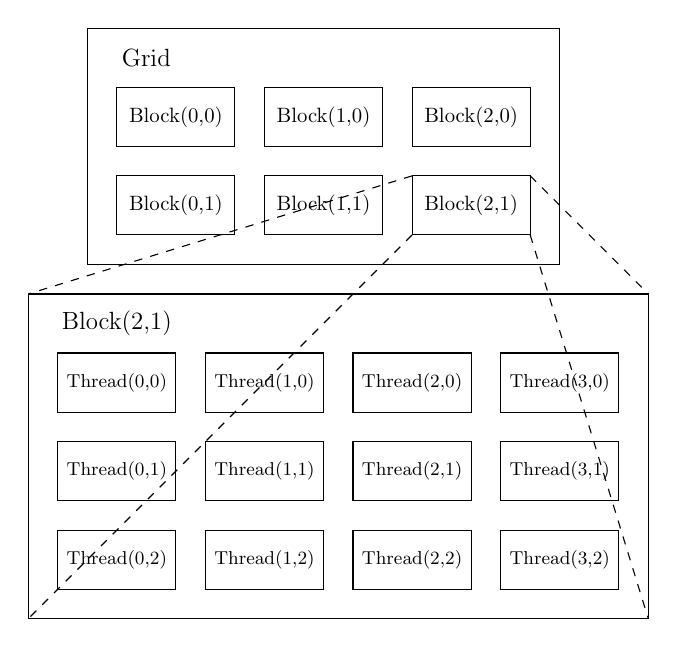
\begin{tikzpicture}[scale=0.75, transform shape]
\def\TextBox#1#2#3{
\draw  (#1,#2) rectangle (#1+2,#2+1);
\node at (#1+1, #2+0.5) {#3};
}

\foreach \x in {0,...,2}
  \foreach \y in {0,...,1}
  {
    \TextBox{\x*2.5+1}{-\y*1.5+3}{Block(\x,\y)}
  }
\draw  (0.5,5) rectangle (8.5,1);
\node at (1.5,4.5) {\large Grid};

\foreach \x in {0,...,3}
  \foreach \y in {0,...,2}
  {
    \TextBox{\x*2.5}{-\y*1.5-1.5}{\small Thread(\x,\y)}
  }
\draw  (-0.5,0.5)  rectangle (10,-5);
\node at (1,0) {\large Block(2,1)};

\draw [dashed]  (6,2.5) edge (-0.5,0.5);
\draw [dashed]  (8,2.5) edge (10,0.5);
\draw [dashed]  (6,1.5) edge (-0.5,-5);
\draw [dashed]  (8,1.5) edge (10,-5);
\end{tikzpicture}
\caption[线程组层次结构示意图]{\label{fig:gpu.cuda.blocks}线程组层次结构示意图
\cite{cudadoc-cprogrammingguide}}
\end{figure}

同一个global函数调用时所涉及的线程均使用global函数的参数作为输入,
CUDA提供threadIdx、blockIdx等变量在代码中区分各个线程。
线程以Block为单元分配给GPU上的各个SMX独立执行,
Block之间没有任何直接的同步方式,
程序员不需要知道也不应该猜测各Block是如何在各个SMX执行的。
需要说明的是:强行使用显存作为Block间的同步可能会导致各SMX死锁。
实际Block间同步的最主要方式就是等待该global函数执行完,
此时所有Block状态都是确定的,即已经执行完。

这样GPU或驱动就可以根据实际GPU核心上的SMX数量来具体配置各Block是如何在SMX上执行的,
使得当SM数量不超过Block数量时global函数有了一定的并行扩展性,
见\floatref{fig:gpu.cuda.scalability}。
由于每个Block是运行在一个实际SMX上的,
所以SMX的寄存器、共享存储空间等资源会对Block的大小(包含的Thread数量)有一定的限制,
而CUDA对Grid大小(包含的Block数量)的限制则很小。
NVIDIA这样做是为了通过强制程序员对计算任务进行分割的方式获得了一定的程序并行扩展性,
同时也简化了同一系列不同规格GPU的设计,即通过增减SMX的数量来控制GPU计算能力。

\begin{figure}
\centering
\begin{tikzpicture}[scale=0.6, transform shape]
\def\TextBox#1#2#3{
\draw  (#1,#2) rectangle (#1+2,#2+1);
\node at (#1+1, #2+0.5) {#3};
}

\foreach \x in {0,...,3}
  \foreach \y in {0,...,1}
  {
    \TextBox{\x*2.5+1}{-\y*1.5+3}{Block(\x,\y)}
  }
\draw  (0.5,5) rectangle (11,1);
\node at (3,4.5) {\large Kernel函数的Grid};

\draw [dashed] (-3,-4) -- (16.5,-4);

\draw  (-1,-3.5) rectangle (4.5,-1);
\node at (1.5,-1.5) {\large 2个SMX的GPU};
\draw [-latex new, arrow head=3mm] (7,1) -- (9.5,-1);
\foreach \x in {0,...,1}
{
  \TextBox{\x*2.5-0.5}{-3}{SMX \x}
}
\foreach \t in {0,...,3}
{
  \foreach \x in {0,...,1}
  {
    \TextBox{\x*2.5-0.5}{-\t*2-6}{Block(\t,\x)}
  }
  \draw  (-1,-\t*2-4.75) rectangle (4.5,-\t*2-6.25);
}

\draw  (5.5,-3.5) rectangle (16,-1);
\node at (8,-1.5) {\large 4个SMX的GPU};
\draw [-latex new, arrow head=3mm] (3.5,1) -- (2,-1);
\foreach \x in {0,...,3}
{
  \TextBox{\x*2.5+6}{-3}{SMX \x}
}
\foreach \t in {0,...,1}
{
  \foreach \x in {0,...,3}
  {
    \TextBox{\x*2.5+6}{-\t*2-6}{Block(\x,\t)}
  }
  \draw  (5.5,-\t*2-4.75) rectangle (16,-\t*2-6.25);
}

\draw [dashed,-latex new, arrow head=3mm] (-1.5,-4.5) -- (-1.5,-13);
\foreach \t in {0,...,3}
{
  \node at  (-2.5,-\t*2-5.5) {\Large t=\t};
}

\draw (5,-0.5) -- (5,-12.5);
\end{tikzpicture}
\caption[CUDA程序的扩展性示意图]{\label{fig:gpu.cuda.scalability}CUDA程序的扩展性示意图
\cite{cudadoc-cprogrammingguide}}
\end{figure}

总的来说,GPU核心相当于一组不能单独编程的、以显存作为共享存储器的、带有自动负载平衡的小型向量机组。


\subsection{CUDA的GPU设备模型}

\begin{figure}
\centering
\begin{tikzpicture}[scale=0.75, transform shape]
%15*SMX
\def\SMX#1#2{
\draw  (#1+0, #2) rectangle (#1+1, #2+1);
\node at (#1+0.5, #2+0.5) {\small SMX};
}
\def\len{1.5}
\foreach \x in {0,...,8}
{ \SMX{\x*\len}{0} }
\foreach \x in {0,...,7}
{ \SMX{\x*\len+0.75}{-3} }

%L2 Cache
\draw  (0,-0.5) rectangle (13,-1.5);
\node at (6.5,-1) {L2缓存};


\def\Memory#1#2{
\draw  (#1,#2) rectangle (#1+2,#2+1);
\node at (#1+1,#2+0.5) {\small 显存控制器};
}
\foreach \i in {0,1,2}
{ \Memory{-2.5}{-\i*1.5} }
\foreach \i in {0,1,2}
{ \Memory{13.5}{-\i*1.5} }

\draw  (-2.5,2) rectangle (15.5,1.5);
\node at (6.5,1.75) {线程调度器(GigaThread Engine)};

\draw  (-2.5,3) rectangle (15.5,2.5);
\node at (6.5,2.75) {PCI Express 3.0接口};

\draw  (-3,4) rectangle (16,-3.5);
\node at (-1.5,3.5) {\Large GK110};
\end{tikzpicture}
\caption[GK110结构示意图]{\label{fig:gpu.cuda.gk110}GK110结构示意图
\cite{cudadoc-KeplerGK110ArchitectureWhitepaper}}
\end{figure}

GPU是由多个SMX组成的,例如Kepler架构GK110核心
(见\floatref{fig:gpu.cuda.gk110})就包含15个SMX,
其中每个SMX(见\floatref{fig:gpu.cuda.smx})
含有192个CUDA Core单元(支持单精度、整数计算,图示中Core)、
64个双精度浮点计算单元(图示中DP Unit)、
32个特殊函数计算单元(图示中SFU)、
32个读取/存储单元(图示中LD/ST),
4个Wrap调度器,65536个32bit寄存器。
SMX以32个Thread为一组(称为wrap)来调度Block中的线程,
每个SMX有4个wrap调度器和8个指令分派单元,这使得SMX可以同时执行4个wrap,
每个周期中每个wrap最多可以有两条不相关的指令被同时分派。
\cite{cudadoc-KeplerGK110ArchitectureWhitepaper}

\begin{figure}
\centering
%\includegraphics[scale=0.6]{smx.png}
\begin{tikzpicture}[scale=0.7, transform shape]
\def\TextBox#1#2#3#4
{
  \draw (#1,#2) rectangle (#1+#3,#2+1);
  \node at (#1+#3/2, #2+0.5) {#4};
}

\def\CoreLine#1#2
{
\foreach \i in {0,...,2}
{ \TextBox{#1+\i*1.5+0}{#2+0}{1}{Core} }
\TextBox{#1+4.5}{#2+0}{2}{DP Unit}

\foreach \i in {0,...,2}
{ \TextBox{#1+\i*1.5+7}{#2+0}{1}{Core} }
\TextBox{#1+11.5}{#2+0}{2}{DP Unit}

\TextBox{#1+14}{#2+0}{1.5}{LD/ST}
\TextBox{#1+16}{#2+0}{1}{SFU}
}

\CoreLine{0}{0}

\CoreLine{0}{-4}

\draw [decorate, decoration={brace, amplitude=10pt}] (-0.5,-4.25) -- (-0.5,1.25);
\node [left]at (-1,-1.5) {\large 32组};
\draw [loosely dashed] (0.5,-0.5) -- (0.5,-2.5);
\draw [loosely dashed] (8,-0.5) -- (8,-2.5);
\draw [loosely dashed] (16.5,-0.5) -- (16.5,-2.5);

\draw  (-0.5,2.5) rectangle (17.5,1.5);
\node at (8,2) {\large 寄存器文件(65536个 32bit寄存器)};

\foreach \x in {0,...,3}
{
  \def\xlen{4.5}
  \draw  (\x*\xlen-0.25,4) rectangle (\x*\xlen-0.25+4,3);
  \node  at (\x*\xlen+1.75,3.5) {\large Wrap调度器}; 
}
\draw  (-0.5,4.5) rectangle (17.5,5.5);
\node at (8,5) {\large 指令缓存};

\draw  (17.5,-4.5) rectangle (-0.5,-5.5);
\draw  (17.5,-6) rectangle (-0.5,-7);
\draw  (17.5,-7.5) rectangle (-0.5,-8.5);
\node at (8,-5) {\large 内部互联网络};
\node at (8,-6.5) {\large 64KB 共享存储区 / L1 缓存};
\node at (8,-8) {\large 48KB 只读数据缓存};

\foreach \x in {0,...,7}
{
  \foreach \y in {0,1}
  {
    \draw  (\x*2.25-0.5,-\y*1.5-9) rectangle (\x*2.25+1.5,-\y*1.5-10);
    \node at (\x*2.25+0.5,-\y*1.5-9.5) {纹理单元};
  }
}

\draw  (-3,-12) rectangle (18,6.5);
\node [right] at (-2.5,6) {\Large SMX};
\end{tikzpicture}
\caption[SMX结构示意图]{\label{fig:gpu.cuda.smx}SMX结构示意图
\cite{cudadoc-KeplerGK110ArchitectureWhitepaper}}
\end{figure}

SMX的存储器结构较为复杂,通用存储器的结构见\floatref{fig:gpu.cuda.memory},
其中寄存器部分和传统程序一样,并不直接对程序员可见,由CUDA编译器进行分配,
L1缓存、L2缓存对程序员也不是直接可见的,会在访问显存时自动进行调度。

\begin{figure}
\centering
\begin{tikzpicture}[scale=0.8, transform shape]

\draw  (0,3) ellipse (1 and 0.5);
\node at (0,3) {Thread};

\draw  (-1.5,0.5) rectangle (1.5,1.5);
\node at (0,1) {L1缓存};

\draw  (-5,0.5) rectangle (-2,1.5);
\node at (-3.5,1) {共享存储区};

\draw  (2,0.5) rectangle (5,1.5);
\node at (3.5,1) {只读数据缓存};

\draw [latex new-latex new, arrow head=3mm] (0,2.5) -- (0,1.5);
\draw [latex new-latex new, arrow head=3mm] (-0.5,2.5) -- (-3.5,1.5);
\draw [latex new-, arrow head=3mm] (0.5,2.5) -- (3.5,1.5);

\draw  (-5,-1.5) rectangle (5,-0.5);
\node at (0,-1) {\large L2缓存};
\draw [latex new-latex new, arrow head=3mm](0,0.5) -- (0,-0.5);
\draw [latex new-, arrow head=3mm](3.5,0.5) -- (3.5,-0.5);

\draw  (-5,-3.5) rectangle (5,-2.5);
\node at (0,-3) {\large 显存};
\draw [latex new-latex new, arrow head=3mm](0,-1.5) -- (0,-2.5);

\draw [decorate, decoration={brace, amplitude=7pt}] (-5.5,0) -- (-5.5,4);
\node [left] at (-5.75,2) {\large SMX};

\draw [decorate, decoration={brace, amplitude=7pt}] (-7,-2) -- (-7,4);
\node [left] at (-7.5,1) {\large GK110};

\draw (-5,2.5) rectangle (-2,3.5);
\node at (-3.5,3) {寄存器};
\draw [latex new-latex new, arrow head=3mm] (-1,3) -- (-2,3);
\end{tikzpicture}
\caption[Kepler存储器结构示意图]{\label{fig:gpu.cuda.memory}Kepler存储器结构示意图
\cite{cudadoc-KeplerGK110ArchitectureWhitepaper}}
\end{figure}

Global函数和device函数可以通过指针直接访问共享存储区、显存。
共享存储区位于SMX内,和L1缓存共用64KB空间,
在global函数启动时可以对共享存储区/L1缓存的分配进行设置,
分配的方式有:16KB/48KB、32KB/32KB(限Kepler架构)、48KB/16KB三种。
\cite{cudadoc-KeplerGK110ArchitectureWhitepaper}

在SMX上运行的Block中的所有线程共享SMX全部的65536个32位寄存器,
一旦分配完成,每个Thread线程就只能使用自己所有的寄存器,其他的寄存器则不可见。
每个Thread需要使用的寄存器数量由CUDA编译器控制。

共享存储区则对同一个Block内所有的线程可见,是同一个Block内的Thread协作、通讯的主要方式,
每个Block使用的共享存储区的大小在global函数启动时进行配置。

只读数据缓存可以用来加速在global函数运行过程中保持不便的数据的读取,
程序员可以通过带有const  \_\_restrict\_\_标识的指针进行访问,
也可以通过纹理模式访问。在Fermi及之前的架构中,该部分缓存只能通过纹理方式使用。
\cite{cudadoc-KeplerGK110ArchitectureWhitepaper}



\section{其他GPU编程技术简介}

\subsection{OpenCL}

在以CUDA为代表的各种硬件相关的GPU、众核编程技术发展之后,
苹果公司提出异构平台计算的开放标准OpenCL,
标准文本见文献\onlinecite{opencl}。

在GPU通用计算领域起步较晚的AMD公司(原ATI公司被AMD收购)
放弃设计一个CUDA这样专为自己生产的GPU编程的编程技术,
直接采用OpenCL作为其GPU的主要开发技术。

OpenCL在很多设备概念、编程模型上照搬较为成熟的CUDA的设计,
但和CUDA相比仍有较大差异。
CUDA程序的编译过程主要发生在主程序开发过程中,CUDA C/C++编译器首先处理CUDA程序的源代码,
把代码分为GPU端和CPU端两部分,CPU端的代码交给GCC/MSVC等传统编译器进行编译,
GPU端的代码则由自己处理,生成相应的GPU PTX代码、主机端调用代码等部分,
最后和程序的其他部分链接成一个主程序。
这其中的PTX代码类似“GPU上的汇编代码”,实际上更接近于Java编译后的字节码,
PTX代码在运行时由主机端驱动程序编译成实际GPU的硬件指令交给GPU运行。
通过增加PTX这一层抽象,NVIDIA使得程序能够在GPU ISA(Instruction Set Architecture)
设计发生变化时仍然可以直接运行。

OpenCL代码语法和CUDA一样\footnote{CUDA后期加入了C++支持。}以
C语言为蓝本\footnote{现在也有为OpenCL增加C++支持的提议,%
见文献\onlinecite{gaster2013opencl}。},
但并不和普通的C代码混在一起,
而是直接以文本形式保存于程序或其他数据文件中,
在运行时由硬件驱动进行编译生成实际硬件代码运行。
所以说OpenCL程序的编译过程主要发生在运行时。

现在支持OpenCL的主要硬件/厂商有:\cite{opencl-conformant-products}
\begin{enumerate}[1)]
\item Intel x86 CPU(及内嵌的Intel HD Graphics集成显卡)
\item AMD CPU/APU
\item AMD显卡
\item NVIDIA显卡
\item Intel MIC(Many Integrated Core) Architecture
\item ARM
\end{enumerate}
相对来说,AMD显卡和MIC上的OpenCL支持较好,因为这是它们上的主要编程方式,
NVIDIA对OpenCL的支持略差,某些情况下可能会有性能明显下降的情况。


\subsection{C++ AMP}

C++ AMP全称C++ Accelerated Massive Parallelism,是微软提出的一个开放的C++ GPU编程标准,
并给出了Windows平台上基于DirectX 11的实现。
C++ AMP的标准文本见文献\onlinecite{cppamp}。
C++ AMP和CUDA类似,都是在已有的语言上增加了新的部分来对GPU进行编程。
\cite{cppamp-overview}

由于C++ AMP是一个开放标准,所以也可能会有进一步的发展。
2012年Intel公司展示了一个把C++ AMP代码编译到OpenCL的实现,使得C++ AMP跨系统跨平台成为可能。
\cite{cppamp-opencl}
不过暂时还没有该技术转化为产品的消息。
在Intel之后,LLVM社区中也出现了一个把C++ AMP代码编译到OpenCL的开源实现\cite{llvm-amp-opencl-prototype}。


\subsection{OpenACC与OpenMP}

由于之前的GPU编程技术需要程序员管理的细节过多,
在2011年11月有CAPS、CRAY、NVIDIA和PGI等公司联合提出了并行计算标准OpenACC。
\cite{reyes2012comparative}
OpenACC标准文本可以从\url{http://www.openacc-standard.org/Downloads}下载。
OpenACC与OpenMP类似,是一种基于用户制导语句的半自动并行化标准。
OpenMP主要针对于共享存储器的CPU多核环境,
而OpenACC则主要面向CPU+GPU异构环境。

当前支持OpenACC的编译器主要为CAPS、CRAY、PGI等公司提供的也商业编译器。

OpenACC已计划被纳入OpenMP 4.0标准。\cite{beyer2011openmp}



\section{GPU线性方程组求解算法简介}

数值计算中线性方程组的求解方法基本可以分为两大类:直接解法和迭代解法。
直接解法的计算量固定且容易估计,没有迭代收敛性问题,但算法本身并行度太低,
很难适合GPU这样的类向量机型处理器,所以以下主要介绍迭代解法。

\subsection{传统迭代算法简介}
考虑如下形式的线性方程组
\begin{align}
  \bm{A}\bm{x}=\bm{b}
\end{align}
其中
\begin{align}
  \bm{A}=\begin{pmatrix}
  a_{11} & a_{12} & \cdots & a_{1n}\\
  a_{21} & a_{22} & \cdots & a_{2n}\\
  \vdots & \vdots & \ddots & \vdots\\
  a_{n1} & a_{n2} & \cdots & a_{nn}\\
  \end{pmatrix}
\end{align}
并记
\begin{align}
  \bm{D}=\begin{pmatrix}
      a_{11} &  &  & \\
       & a_{22} &  & \\
       &  & \ddots & \\
       &  &  & a_{nn}\\
      \end{pmatrix}
  \hspace{5pt}
  \bm{L}=\begin{pmatrix}
    0 &  &  & \\
    a_{21} & 0 &  & \\
    \vdots & \ddots & 0 & \\
    a_{n1} & \cdots & a_{n,n-1} & 0\\
    \end{pmatrix}
  \hspace{5pt}
  \bm{U}=\begin{pmatrix}
      0 & a_{12} & \cdots & a_{1n}\\
       & 0 & \ddots & \vdots\\
       &  & 0 & a_{n-1,n}\\
       &  &  & 0\\
      \end{pmatrix}
\end{align}

\subsubsection{Jacobi迭代}
Jacobi迭代的形式为
\begin{align}
  \bm{x}^{(k+1)}=\bm{D}^{-1}\pb[b]{\bm{b}-\pb{\bm{L}+\bm{U}}\bm{x}^{(k)}}
\end{align}
收敛条件为
\begin{align}
  \rho\pb[b]{\bm{D}^{-1}\pb{\bm{L}+\bm{U}}}<1
\end{align}
其中$\rho(\bm{M})$表示$\bm{M}$的谱半径。\cite{golub2012matrix}

\subsubsection{Gauss-Seidel迭代}
Gauss-Seidel迭代的形式为
\begin{align}
  \bm{x}^{(k+1)}=\pb{\bm{L}+\bm{D}}^{-1}\pb[b]{\bm{b}-\bm{U}\bm{x}^{(k)}}
\end{align}
当$\bm{A}$对称正定时,Gauss-Seidel迭代收敛。\cite{golub2012matrix}

Gauss-Seidel迭代在传统CPU求解线性方程组中使用广泛,
但其主要步骤$\pb{\bm{L}+\bm{D}}^{-1}$项的计算是一个串行过程,
较难在GPU这种向量机上实现,所以在GPU求解线性方程组中使用不多。

\subsubsection{逐次超松弛迭代}
逐次超松弛迭代是Jacobi迭代和Gauss-Seidel迭代的推广,
其迭代的形式为\cite{golub2012matrix}
\begin{align}
  \bm{x}^{(k+1)}=\pb{\bm{L}+\omega\bm{D}}^{-1}
                  \pb[b]{\omega\bm{b}-\pb{\omega\bm{U}+(\omega-1)\bm{D}}\bm{x}^{(k)}}
\end{align}

该迭代方法在GPU上面临和Gauss-Seidel迭代同样的问题。

\subsection{Krylov子空间类算法简介}
\subsubsection{CG(Conjugate gradient)共轭梯度法}
CG方法可以用于求解$\bm{A}$对称正定时的线性方程,
其求解过程见\floatref{alg:gpu.cg}。\cite{golub2012matrix}

\begin{algorithm}
\KwIn{$\bm{A},\bm{x}_0,\bm{b}$}
\KwOut{$\bm{x}_e$}
$\bm{r}_0 := \bm{b}-\bm{A}\bm{x}_0$ \;
$\bm{p}_0 := \bm{r}_0$\;
$k:=0$\;

\While{ True }{
$\displaystyle \alpha_k:=\frac{\bm{r}_k^T\bm{r}_k}{\bm{p}_k^T\bm{A}\bm{p}_k}$\;
$\bm{x}_{k+1}:=\bm{x}_k+\alpha_k\bm{p}_k$\;
$\bm{r}_{k+1}:=\bm{r}_k-\alpha_k\bm{A}\bm{p}_k$\;
\If{$\vb{\bm{r}_{k+1}}$ is small}{
  return $\bm{x}_e := \bm{x}_{k+1}$\;
}
$\displaystyle \beta_k := \frac{\bm{r}_{k+1}^T\bm{r}_{k+1}}{\bm{r}_k^T\bm{r}_k}$\;
$\bm{p}_{k+1}:=\bm{r}_{k+1}+\beta_k\bm{p}_k$\;
$k:=k+1$\;
}
\setlabelname{CG方法}
\caption{CG方法\label{alg:gpu.cg}}
\end{algorithm}

带预条件的CG方法见\floatref{alg:gpu.pcg}。\cite{golub2012matrix}
由于只需在在\floatref{alg:gpu.pcg}中令$\bm{M}=\bm{I}$即可得到\floatref{alg:gpu.cg},
所以以下只给出带预条件的迭代算法。

\begin{algorithm}
\KwIn{$\bm{A},\bm{x}_0,\bm{b},\bm{M}$}
\KwOut{$\bm{x}_e$}
$\bm{r}_0 := \bm{b}-\bm{A}\bm{x}_0$ \;
$\bm{z}_0 := \bm{M}^{-1}\bm{r}_0$\;
$\bm{p}_0 := \bm{r}_0$\;
$k:=0$\;
\While{ True }{
$\displaystyle \alpha_k:=\frac{\bm{r}_k^T\bm{z}_k}{\bm{p}_k^T\bm{A}\bm{p}_k}$\;
$\bm{x}_{k+1}:=\bm{x}_k+\alpha_k\bm{p}_k$\;
$\bm{r}_{k+1}:=\bm{r}_k-\alpha_k\bm{A}\bm{p}_k$\;
\If{$\vb{\bm{r}_{k+1}}$ is small}{
  return $\bm{x}_e := \bm{x}_{k+1}$\;
}
$\bm{z}_{k+1}:=\bm{M}^{-1}\bm{r}_{k+1}$\;
$\displaystyle \beta_k := \frac{\bm{z}_{k+1}^T\bm{r}_{k+1}}{\bm{z}_k^T\bm{r}_k}$\;
$\bm{p}_{k+1}:=\bm{z}_{k+1}+\beta_k\bm{p}_k$\;
$k:=k+1$\;
}
\setlabelname{带预条件的CG方法}
\caption{\label{alg:gpu.pcg}带预条件的CG方法}
\end{algorithm}

\subsubsection{BiCGStab}
对于非对称正定的方程组,可以把CG方法扩展为BiCG(BiConjugate Gradient)方法。
\cite{press2007numericalrecipes}
但由于BiCG方法的数值稳定性较差,可能会遇到不收敛的情况,
所以文献\onlinecite{van1992bicgstab}提出了BiCGStab方法,
见\floatref{alg:gpu.pbicgstab}。

\begin{algorithm}
\KwIn{$\bm{A},\bm{x}_0,\bm{b},\bm{K}$}
\KwOut{$\bm{x}_e$}

$\bm{r}_0 := \bm{b}-\bm{A}\bm{x}_0$ \;
任取$\bm{r}_0^*$使得$\bm{r}_0^*\cdot\bm{r}_0\neq 0$\;
$\rho_0:=\alpha:=\omega_0:=1$\;
$\bm{v}_0:=\bm{p}_0 := \bm{0}$\;
$k:=1$\;
\While{ True }{
$\rho_k:=\bm{r}_0^*\cdot\bm{r}_{k-1}$\;
$\displaystyle \beta:=\frac{\rho_k}{\rho_{k-1}}\frac{\alpha}{\omega_{k-1}}$\;
$\bm{p}_k:=\bm{r}_{k-1}+\beta\pb{\bm{p}_{k-1}-\omega_{k-1}\bm{v}_{k-1}}$\;
$\bm{y}:=\bm{K}^{-1}\bm{p}_k$\;
$\bm{v}_k:=\bm{Ay}$\;
$\displaystyle \alpha:=\frac{\rho_k}{\bm{r}_0^*\cdot\bm{v}_k}$\;
$\bm{s}:=\bm{r}_{k-1}-\alpha\bm{v}_k$\;
$\bm{z}:=\bm{K}^{-1}\bm{s}$\;
$\bm{t}:=\bm{Az}$\;
$\displaystyle \omega_k:=\frac{(\bm{K}^{-1}\bm{t})\cdot(\bm{K}^{-1}\bm{s})}{(\bm{K}^{-1}\bm{t})\cdot(\bm{K}^{-1}\bm{t})}$\;
$\bm{x}_{k}:=\bm{x}_{k-1}+\alpha\bm{y}+\omega_k\bm{z}$\;
end\;
\If{$\bm{x}_{k}$收敛}{
  return $\bm{x}_e := \bm{x}_{k}$\;
}
$\bm{r}_k:=\bm{s}-\omega_k\bm{t}$\;
$k:=k+1$\;
}
\setlabelname{带预条件的BiCGStab方法}
\caption{\label{alg:gpu.pbicgstab}带预条件的BiCGStab方法}
\end{algorithm}

\subsubsection{GMRES(Generalized Minimal RESidual method)广义最小残量法}
GMRES是一种可以用于求解非对阵矩阵的Krylov子空间方法,
由Saad和Schultz在1986年提出。\cite{saad1986gmres}

实际计算中GMRES需要再启动等技巧,这里只给出一个简单的GMRES算法,
见\floatref{alg:gpu.gmres}。\cite{golub2012matrix}

\begin{algorithm}
\KwIn{$\bm{A},\bm{x}_0,\bm{b}\text{,并有}\bm{A}\bm{x}_0\approx\bm{b}$}
\KwOut{$\bm{x}_e$}

$\bm{r}_0 := \bm{b}-\bm{A}\bm{x}_0$ \;
$h_{10}:=\| \bm{r}_0\|_2$\;
$k:=0$\;
\While{ $h_{k+1,k}>0$ }{
$\displaystyle \bm{q}_{k+1}:=\frac{\bm{r}_k}{h_{k+1,k}}$\;
$k:=k+1$\;
$\bm{r}_k:=\bm{A}\bm{q}_k$\;
\For{$i:=1 \  \mathrm{to} \   k$}
{
$h_{ik}:=\bm{q}_i^T\cdot\bm{r}_k$\;
$\bm{r}_k:=\bm{r}_k-h_{ik}\bm{q}_i$\;
}
$h_{k+1,k}:=\| \bm{r}_k\|_2$\;
$\bm{x}=\bm{x}_0+\bm{Q}_k\bm{y}_k$
其中$\bm{y}_k$使$\left\| h_{10}e_1-\overline{\bm{H}_m}\bm{y}_k \right\|_2$最小\;
}
$\bm{x}_e:=\bm{x}_k$\;
\setlabelname{GMRES方法}
\caption{\label{alg:gpu.gmres}GMRES方法}
\end{algorithm}


\subsection{预条件处理简介}
当矩阵$\bm{A}$的条件数较大时,以上的各种迭代方法的收敛速度往往并不理想,
为了改善在大条件数情况下的收敛速度,Krylov往往和预条件处理共同使用。
预条件处理的思路是把原始问题同解变换为一个条件数较小的问题。
预条件的方法一般是找到一个矩阵$\bm{P}$使得$\bm{P^{-1}A}$的条件数较小,
且方程组$\bm{Px}=\bm{b}$较容易求解。\cite{saad2003iterative}

以下列举一些常见的预条件算法
\begin{enumerate}
\item Jacobi,又称对角线预处理

取\cite{saad2003iterative}
\begin{align}
  \bm{P}=\begin{pmatrix}
  \displaystyle \frac{1}{A_{11}} & & &\\
  & \displaystyle \frac{1}{A_{22}} & &\\
  & & \ddots &\\
  & & & \displaystyle \frac{1}{A_{nn}}\\
  \end{pmatrix}
\end{align}

\item SPAI(SParse Approximate Inverse)\cite{saad2003iterative}

计算使$\|\bm{AT}-\bm{I}\|_F$最小的$\bm{T}$,
取$\bm{P}=\bm{T}^{-1}$,具体过程参见文献\onlinecite{grote1997parallel}。
由于在计算中只使用$\bm{P}^{-1}$,所以不需要计算$\bm{T}^{-1}$。

\item IC(Incomplete Cholesky factorization)

参见文献\onlinecite{golub2012matrix}第10.3.2节。

\item ILU(Incomplete LU Factorizations)

参见文献\onlinecite{saad2003iterative}第10.3节。

\end{enumerate}
上面介绍的预条件算法除了Jacobi具有天然的并行度外,
其他算法的Setup过程的串行度较高,较难在GPU上实现。


%\subsubsection{多重网格}

\begin{table}
\centering
\caption{不同求解算法求解2维Poisson问题需要的计算量\cite{trottenberg2000multigrid}}
\begin{minipage}{.7\linewidth}
\centering
\begin{tabular}{lc}
\toprule
求解方法 & 需要的计算量\footnote{记N为未知元数量。}\\
\midrule
高斯消去 & $\mathcal{O}(N^2)$\\
Jacobi迭代 & $\mathcal{O}(N^2\log\epsilon)$\\
Gauss-Seidel迭代 & $\mathcal{O}(N^2\log\epsilon)$\\
超松弛迭代 & $\mathcal{O}(N^{3/2}\log\epsilon)$\\
CG & $\mathcal{O}(N^{3/2}\log\epsilon)$\\
IC CG & $\mathcal{O}(N^{5/4}\log\epsilon)$\\
ADI\footnote{Alternating Direction Implicit,交替隐式迭代。} & $\mathcal{O}(N\log N)$\\
完全多重网格法 & $\mathcal{O}(N)$\\
\bottomrule
\end{tabular}
\end{minipage}
\end{table}


\subsection{常见存储格式介绍}

\subsubsection{坐标格式(COO)}
COO格式直接存储每个非零元素的位置和值,
如矩阵
\begin{align*}
\bm{A}=\begin{pmatrix}
1 & 7 & 0\\
0 & 2 & 0\\
5 & 0 & 3
\end{pmatrix}
\end{align*}
的COO格式表示为\footnote{下标从0开始计数,下同。}
\begin{align*}
\mathrm{rows}=\begin{pmatrix}
0 & 0 & 1 & 2 & 2  
\end{pmatrix}
\\
\mathrm{cols}=\begin{pmatrix}
0 & 1 & 1 & 0 & 2
\end{pmatrix}
\\
\mathrm{values}=\begin{pmatrix}
1 & 7 & 2 & 5 & 3
\end{pmatrix}
\end{align*}



\subsubsection{行压缩格式(CSC)}
CSC格式把每行的非零元连续存放,相对于COO节省了存储行号的空间,
如矩阵
\begin{align*}
\bm{A}=\begin{pmatrix}
1 & 7 & 0\\
0 & 2 & 0\\
5 & 0 & 3
\end{pmatrix}
\end{align*}
的CSC格式表示为
\begin{align*}
\mathrm{ptr}&=\begin{pmatrix}
0 & 2 & 3  
\end{pmatrix}
\\
\mathrm{cols}&=\begin{pmatrix}
0 & 1 & 1 & 0 & 2
\end{pmatrix}
\\
\mathrm{values}&=\begin{pmatrix}
1 & 7 & 2 & 5 & 3
\end{pmatrix}
\end{align*}

如果把行列的存储方式调换,则可得到另一种格式,即列压缩格式(CSC)。

\subsubsection{对角线格式(DIA)}
对角线格式是专门用于存储对角线稀疏矩阵的一种格式,
其思路是只存储有非零元素的对角线。
如矩阵\cite{bell2008spmv}
\begin{align*}
\bm{A}=\begin{pmatrix}
1 & 7 & 0 & 0\\
0 & 2 & 8 & 0\\
5 & 0 & 3 & 9\\
0 & 6 & 0 & 4
\end{pmatrix}
\end{align*}
的DIA格式表示为\footnote{其中$\_$表示DIA格式不使用的任意值,下同。}
\begin{align*}
\mathrm{data}=\begin{pmatrix}
\_ & 1 & 7\\
\_ & 2 & 8\\
5 & 3 & 9\\
6 & 4 & \_
\end{pmatrix}
\quad
\mathrm{offsets}=\begin{pmatrix}
-2 & 0 & 1\\
\end{pmatrix}
\end{align*}


\subsubsection{ELLPACK格式(ELL)}
ELL是为向量机设计的一种稀疏矩阵存储格式,
用于存储$M\times N$的矩阵且每行最多只有$k$个元素的情况。\cite{grimes1979itpack}
如矩阵\cite{bell2008spmv}
\begin{align*}
\bm{A}=\begin{pmatrix}
1 & 7 & 0 & 0\\
0 & 2 & 8 & 0\\
5 & 0 & 3 & 9\\
0 & 6 & 0 & 4
\end{pmatrix}
\end{align*}
的ELL格式表示为
\begin{align*}
\mathrm{data}=\begin{pmatrix}
1 & 7 & \_\\
2 & 8 & \_\\
5 & 3 & 9 \\
6 & 4 & \_
\end{pmatrix}
\quad
\mathrm{indices}=\begin{pmatrix}
0 & 1 & \_\\
1 & 2 & \_\\
0 & 2 & 3\\
1 & 4 & \_
\end{pmatrix}
\end{align*}

\subsubsection{Hybrid格式(HYB)}
由于ELL格式只适合每行元素个数相差不多的情况,
所以又进一步出现了Hybrid格式,即同时使用ELL格式和COO格式,
ELL格式存储系数矩阵中较为规整的部分(每行元素数量接近),
COO格式则存储剩下的比较不规则的非零元。\cite{bell2008spmv}
如矩阵
\begin{align*}
\bm{A}=\begin{pmatrix}
1 & 7 & 0 & 0\\
0 & 2 & 8 & 0\\
5 & 0 & 3 & 9\\
0 & 6 & 0 & 4
\end{pmatrix}
\end{align*}
可拆分为两个矩阵
\begin{align*}
\bm{A}=\begin{pmatrix}
1 & 7 & 0 & 0\\
0 & 2 & 8 & 0\\
5 & 0 & 3 & 0\\
0 & 6 & 0 & 4
\end{pmatrix}
+
\begin{pmatrix}
0 &  &  & \\
 & 0 &  & \\
 &  & 0 & 9\\
 &  &  & 0
\end{pmatrix}
\end{align*}
分别使用ELL和COO格式进行存储,
ELL格式部分为
\begin{align*}
\mathrm{data}=\begin{pmatrix}
1 & 7\\
2 & 8\\
5 & 3\\
6 & 4
\end{pmatrix}
\quad
\mathrm{indices}=\begin{pmatrix}
0 & 1\\
1 & 2\\
0 & 2\\
1 & 4
\end{pmatrix}
\end{align*}
COO格式部分为
\begin{align*}
\mathrm{rows}=\begin{pmatrix}
2
\end{pmatrix}
\\
\mathrm{cols}=\begin{pmatrix}
3
\end{pmatrix}
\\
\mathrm{values}=\begin{pmatrix}
9
\end{pmatrix}
\end{align*}

HYB格式中,ELL部分每行存储多少个元素不是固定的,
可以根据需要进行变化。

